\documentclass[15pt,a5paper,reqno]{article}
\usepackage{hyperref}
\usepackage[warn]{mathtext}
\usepackage[utf8]{inputenc}
\usepackage[T2A]{fontenc}
\usepackage[russian]{babel}
\usepackage{amssymb, amsmath, multicol}
\usepackage{graphicx}
\usepackage[shortcuts,cyremdash]{extdash}
\usepackage{wrapfig}
\usepackage{floatflt}
\usepackage{lipsum}
\usepackage{verbatim}
\usepackage{concmath}
\usepackage{euler}
\usepackage{xcolor}
\usepackage{etoolbox}
\usepackage{fancyhdr}
\usepackage{subfiles}
\usepackage{enumitem}
\usepackage{amsthm}
\usepackage{indentfirst}
\usepackage{import}

\DeclareMathOperator{\sign}{sign}

\RequirePackage[ left     = 1.5cm,
  right    = 1.5cm,
  top      = 2.0cm,
  bottom   = 1.25cm,
  includefoot,
  footskip = 1.25cm ]{geometry}
\setlength    {\parskip}        { .5em plus .15em minus .08em }
%\setlength    {\parindent}      { .0em }
\renewcommand {\baselinestretch}{ 1.07 }

\fancyhf{}

\renewcommand{\footrulewidth}{ .0em }
\fancyfoot[C]{\texttt{\textemdash~\thepage~\textemdash}}

\makeatletter
\patchcmd\l@section{%
  \nobreak\hfil\nobreak
}{%
  \nobreak
  \leaders\hbox{%
    $\m@th \mkern \@dotsep mu\hbox{.}\mkern \@dotsep mu$%
  }%
  \hfill
  \nobreak
}{}{\errmessage{\noexpand\l@section could not be patched}}
\makeatother
\parindent = 1cm % отступ при красной строке⏎
\pagestyle{fancy}    
\renewcommand\qedsymbol{$\blacksquare$}

\newcommand{\when}[2]{
  \left. #1 \right|_{#2} \hspace
}
\renewcommand{\kappa}{\varkappa}
\RequirePackage{caption2}
\renewcommand\captionlabeldelim{}
\newcommand*{\hm}[1]{#1\nobreak\discretionary{}

\DeclareSymbolFont{T2Aletters}{T2A}{cmr}{m}{it}
{\hbox{$\mathsurround=0pt #1$}}{}}
% Цвета для гиперссылок
\definecolor{linkcolor}{HTML}{000000} % цвет ссылок
\definecolor{urlcolor}{HTML}{799B03} % цвет гиперссылок
 
\hypersetup{pdfstartview=FitH,  linkcolor=linkcolor,urlcolor=urlcolor, colorlinks=true}


%\setcounter{secnum[utf8x]depth}{0}

\begin{document}

% НАЧАЛО ТИТУЛЬНОГО ЛИСТА
\begin{center}
  {\small ФЕДЕРАЛЬНОЕ ГОСУДАРСТВЕННОЕ АВТОНОМНОЕ ОБРАЗОВАТЕЛЬНОЕ\\ УЧРЕЖДЕНИЕ ВЫСШЕГО ОБРАЗОВАНИЯ\\ МОСКОВСКИЙ ФИЗИКО-ТЕХНИЧЕСКИЙ ИНСТИТУТ\\ (НАЦИОНАЛЬНЫЙ ИССЛЕДОВАТЕЛЬСКИЙ УНИВЕРСИТЕТ)\\ ФИЗТЕХ-ШКОЛА РАДИОТЕХНИКИ И КОМПЬЮТЕРНЫХ ТЕХНОЛОГИЙ}\\
  \hfill \break
  \hfill \break
  \hfill \break
  \Huge{Работа 2.1.2. \\ Определение $\frac{C_p}{C_v}$ методом адиабатического расширения газа}\\
\end{center}

\hfill \break
\hfill \break
\hfill \break
\hfill \break
\hfill \break
\hfill \break

\begin{flushright}
  \normalsize{Работу выполнил:}\\
  \normalsize{\textbf{Долгов Александр Алексеевич, группа Б01-106}}\\
\end{flushright}

\begin{center}
  \normalsize{\textbf{Долгопрудный, 2022}}
\end{center}


\thispagestyle{empty} % выключаем отображение номера для этой страницы

% КОНЕЦ ТИТУЛЬНОГО ЛИСТА

\newpage
\thispagestyle{plain}
\tableofcontents
\thispagestyle{plain}
\newpage

\section{Аннотация}

	В данной работе было определено отношение $\frac{C_p}{C_v}$ путём проведения многократных измерений давления в сосуде, наполненном воздухом, над которым совершался адиабатический процесс с последующим нагреванием газа до комнатной температуры.
	
\section{Экспериментальная установка}
	
	В работе используется установка, состоящая из стеклянного сосуда A (объёмом $\approx$ 20 л), снабжённого краном К, U-образного жидкостного манометра. Схема установки показана на рисунке 1. Избыточное давление создаётся с помощью резиновой груши, соединённой с сосудом трубкой с краном $\text{К}_1$
	
	\begin{center}
	    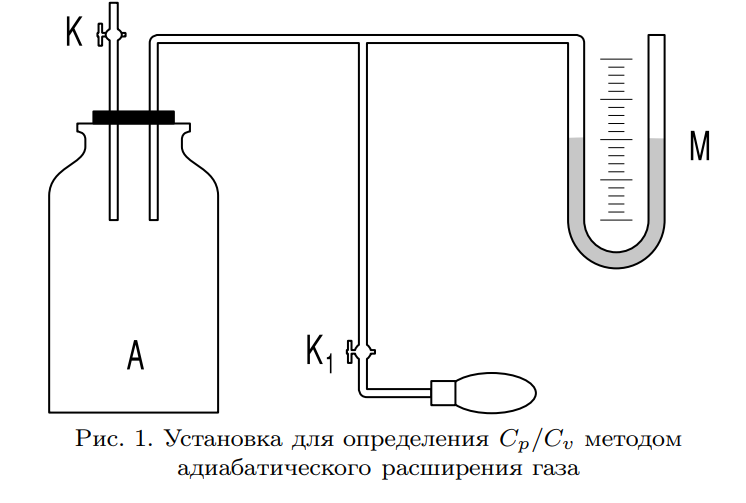
\includegraphics[width = 8cm, height = 5cm]{Рис. 1, Установка.png}
	\end{center}

\section{Теоретические сведения}

    В начале опыта в сосуде находится воздух при комнатной температуре и давлении, превышающем атмосферное. После открытия крана К давление и температура газа будут понижаться. Такой процесс приближённом можно считать адиабатическим. Такое утверждение основано на том, что равновесие по давлению устанавливается значительно быстрее, чем по температуре. Поэтому
    
    \begin{equation}
        \Delta t_P \ll \Delta t_T,
    \end{equation}
    где $\Delta t_P$ и $\Delta t_T$ - соответственно времена выравнивания давления и температуры. 
    
    \noindentЕсли открыть кран К на время $\Delta t$, удовлетворяющее условию:
    
    \begin{equation}
        \Delta t_P \ll \Delta t \ll \Delta t_T
    \end{equation}
	то теплообменом через стенки сосуда за время $\Delta t$ можно пренебречь и считать процесс адиабатическим.
	
	Индексом "1"\>будем обозначать состояние газа после повышения давления с сосуде и выравнивания температуры  с комнатной, индексом "2"\>- сразу после открытия крана и выравнивания давления с атмосферным.
	
	Из уравнения адиабаты и уравнения Менделеева-Клапейрона получим:
	
	\begin{equation}
	    TV^{\gamma - 1} = const, PV = \nu RT \Rightarrow \frac{T^{\gamma}}{P^{\gamma - 1}} = const
	\end{equation}
	
	\noindentОткуда получаем:
	
	\begin{equation}\label{const_S}
	    \left(\frac{P_1}{P_2}\right)^{\gamma - 1} = \left(\frac{T_1}{T_2}\right)^{\gamma}
	\end{equation}
	
	Давление $P_2$ после адиабатического расширения газа равно атмосферному давлению $P_0$, а температура $T_2$ будет ниже комнатной температуры $T_1$.
	
	После того, как кран К будет закрыт, произойдёт медленное изохорное нагревание газа до комнатной температуры со скоростью, определяемой теплопроводностью стеклянных стенок сосуда. Система достигнет равновесия за время порядка $\Delta t_T$. Давление в этом состоянии равно $P_3$. Изохорный процесс описывается законом Гей-Люссака:
	
	\begin{equation}\label{const_V}
	    \frac{P_2}{T_2} = \frac{P_3}{T_1} \Rightarrow \frac{T_1}{T_2} = \frac{P_3}{P_2}
	\end{equation}
	
	\noindentПодставим \eqref{const_V} в \eqref{const_S} и учтём, что $P_2 = P_0$:
	
	\begin{equation}
	    \left(\frac{P_1}{P_0}\right)^{\gamma - 1} = \left(\frac{P_3}{P_0}\right)^{\gamma} \Rightarrow
	\end{equation}
	
	\noindentОтсюда получаем:
	\begin{equation}
	    \gamma = \frac{\ln{(P_1/P_0)}}{\ln{(P_1/P_3)}}
	\end{equation}
	
	В условия данной работы давления $P_1$ и $P_3$ отличаются от атмосферного давления $P_0$ на малую величину, измеряемую жидкостным манометром. Введём обозначения: $P_1 = P_0 + \rho g\Delta h_1$, $P_3 = P_0 + \rho g\Delta h_2$, где $\rho$ - плотность жидкости (воды), $g$ - ускорение свободного падения, $\Delta h_1, \Delta h_2$ - разница в высоте водяных столбов в соседних коленьях манометра.
	
	\begin{equation}
	    \gamma = \frac{ln{(1 + \rho g\Delta h_1/P_0)}}{ln{(1 + \rho g\Delta h_1/P_0)} - ln{(1 + \rho g\Delta h_2/P_0)}} \approx \frac{\Delta h_1}{\Delta h_1 - \Delta h_2}
	\end{equation}
	
	Пусть высота столба воды в колене манометра, соединённом с сосудом равна $h$, а во втором колене - $h'$, тогда справедливы уравнения: $h' - h = \Delta h$ и $h + h' = 2h_0$, где $h_0$ - высота столбов воды в том случае, когда она одинакова для обоих столбов. Отсюда получаем: $\Delta h = 2(h_0 - h)$. В работе производилось измерение именно величины $h$, а не $\Delta h$. Окончательно получаем:
	
	\begin{equation}
	    \gamma = \frac{h_0 - h_1}{h_2 - h_1}
	\end{equation}
	
\section{Оборудование и экспериментальные погрешности}

    В качестве прибора, измеряющего высоту водяного столба использовалась шкала, являющаяся частью U-образной трубки манометра.
    
    \noindent Погрешность измерения данной шкалы равна половине цены деления:
    
    \[\sigma_{h} = 0,5\text{ мм}\]
    
    \noindent Была измерена величина $h_0$:
    \[h_0 = (181.0 \pm 0.5)\text{ мм}\]
    
    Для установления зависимости $h(t)$ использовалась камера мобильного телефона, оборудованная встроенным секундомером. Его погрешностью мы пренебрегаем, так как нахождение зависимости $h(t)$ нужно лишь для оценки порядка величины $\Delta t_T$.
	
\section{Обработка полученных результатов}

    \subsection{Получение оценки для величины $\Delta t_T$}
    
    Сосуда А был наполнен воздухом до давления, превышающего атмосферное. Затем проводилось измерение зависимости высоты $h$ водяного столба в колене, сообщенном с сосудом, от времени. Результаты измерений приведены в таблице 1. и визуально отражены на графике 1. 
    
    Из полученных данных видно, что давление в сосуде перестало понижаться по прошествии времени $\Delta t_T \approx 50\text{ с}$.
    
    \subsection{Измерение показателя адиабаты}
    
    Проводилось 3 серии измерений. В первой кран К открывался приблизительно на время $\Delta t = 0,5$ с, во второй - на $\Delta t = 1$ с, в третьей - на $\Delta t = 1,5$ с. Результаты измерений величин $h_1$, $h_2$, а также результаты расчёта величины $\gamma$ и её погрешности для указанных значений $\Delta t$ приведены в таблице 2. По средним значениям величины $\gamma$ (усреднение по всем измерениям в серии) построен график 1.
    
    Линейной аппроксимацией экспериментальных точек получена зависимость:
    
        \[\gamma = A\Delta t + B\]
        \[A = (-0,063 \pm 0,013) \frac{1}{\text{с}}\]
        \[B = 1,43 \pm 0,01\]
        
    При $\Delta t \approx 0,1\text{ с}$ давление уже почти сравнивается с атмосферным, но теплопроводностью ещё можно пренебречь. Найдём $\gamma (0,1\text{ с})$:
    
    Случайную погрешность величины $\gamma$ найдём по формуле:
    
    \[\sigma_\gamma = \sqrt{\left(\frac{\partial\gamma}{\partial A} \sigma_A\right)^2 + \left(\frac{\partial\gamma}{\partial B} \sigma_B\right)^2} = \sqrt{\left(\sigma_A \Delta t\right)^2 + \left(\sigma_B\right)^2}\]
    
    Систематическую погрешность искать не будем, так как искомое значение $\gamma$ получается экстраполяцией экспериментальных данных.
    
    \[\gamma = \gamma(0,1\text{ с}) \approx 1,43 \pm 0,01\]
    \[\frac{\sigma_\gamma}{\gamma}\approx 0,7\%\]
    
\section{Вывод}

    В ходе данной работы получено значение показателя адиабаты для воздуха. Автором было найдено табличное значение $\gamma = 1,4$ для воздуха при $T = 20^{\circ} C$ (википедия). Таким образом, найденное в работе значения отличается от истинного на $\approx 2\%$, что больше относительной погрешности $\gamma$.
    
    Считаю, что подобное отклонение от "истинного"\> значения вызвано неточностью значений промежутков времени, в течение которых был открыт кран К. Данное время в ходе работы не было измерено точно, а лишь оценивалось по личным ощущениям (в силу малости промежутков времени как-либо их измерить затруднительно). Таким образом, именно погрешность величины $\Delta t$ вносит наибольший вклад в погрешность $\sigma_\gamma$, но этот вклад не был рассчитан.
    
    Для улучшения точности измерений оптимальным вариантом является создание или применение уже готового механизма, который открывал бы кран К (или любым другим способом сообщал бы сосуд с атмосферой) на строго определённое время.
    
\section{Приложения}

    \noindent\textbf{Таблица 1.} Зависимость h(t) после прекращения накачки воздуха\\
    \begin{center}
        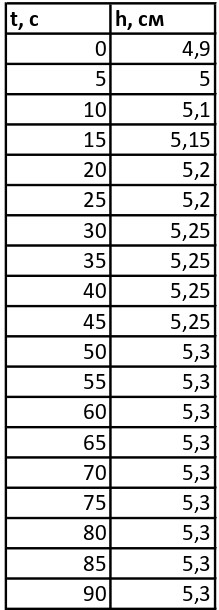
\includegraphics[height = 10cm]{Таблица 1.jpg}
    \end{center}
    
    \newpage
    \noindent\textbf{График 1.} Зависимость h(t) после прекращения накачки воздуха\\
    \begin{center}
        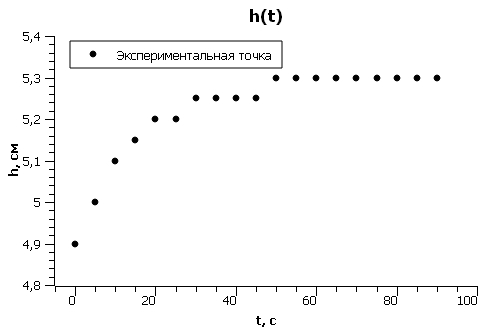
\includegraphics[]{График 1.jpg}
    \end{center}
    
    \newpage
    \noindent\textbf{Таблица 2.} Измерения высоты водяного столба\\
    \begin{center}
        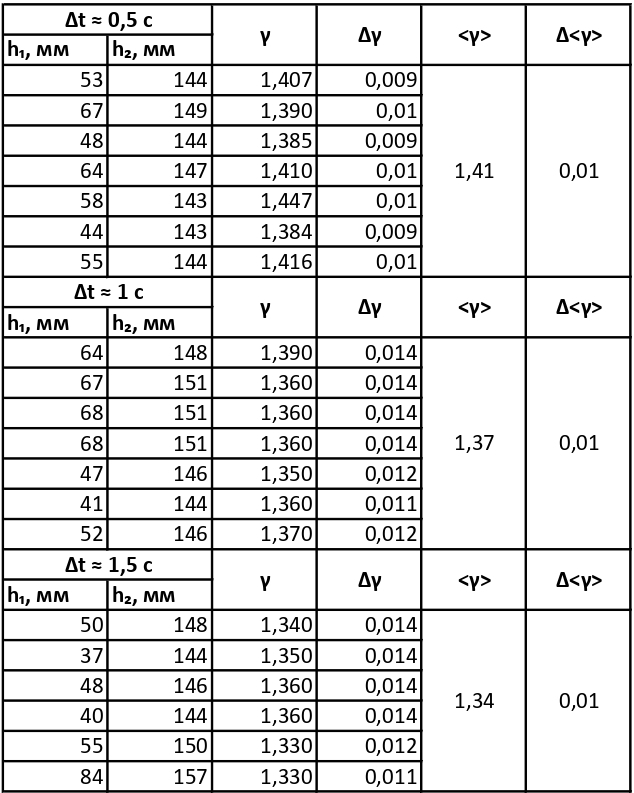
\includegraphics[]{Таблица 2.jpg}
    \end{center}
    
    \newpage
    \noindent\textbf{График 2.} $\gamma(\Delta t)$\\
    \begin{center}
        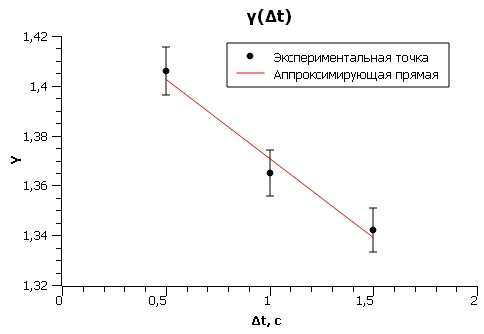
\includegraphics[]{График 2.jpg}
    \end{center}


\end{document}